\blankpage

\thispagestyle{empty}
\clearpage
\begin{tikzpicture}[remember picture, overlay]
\node at (3,-7) {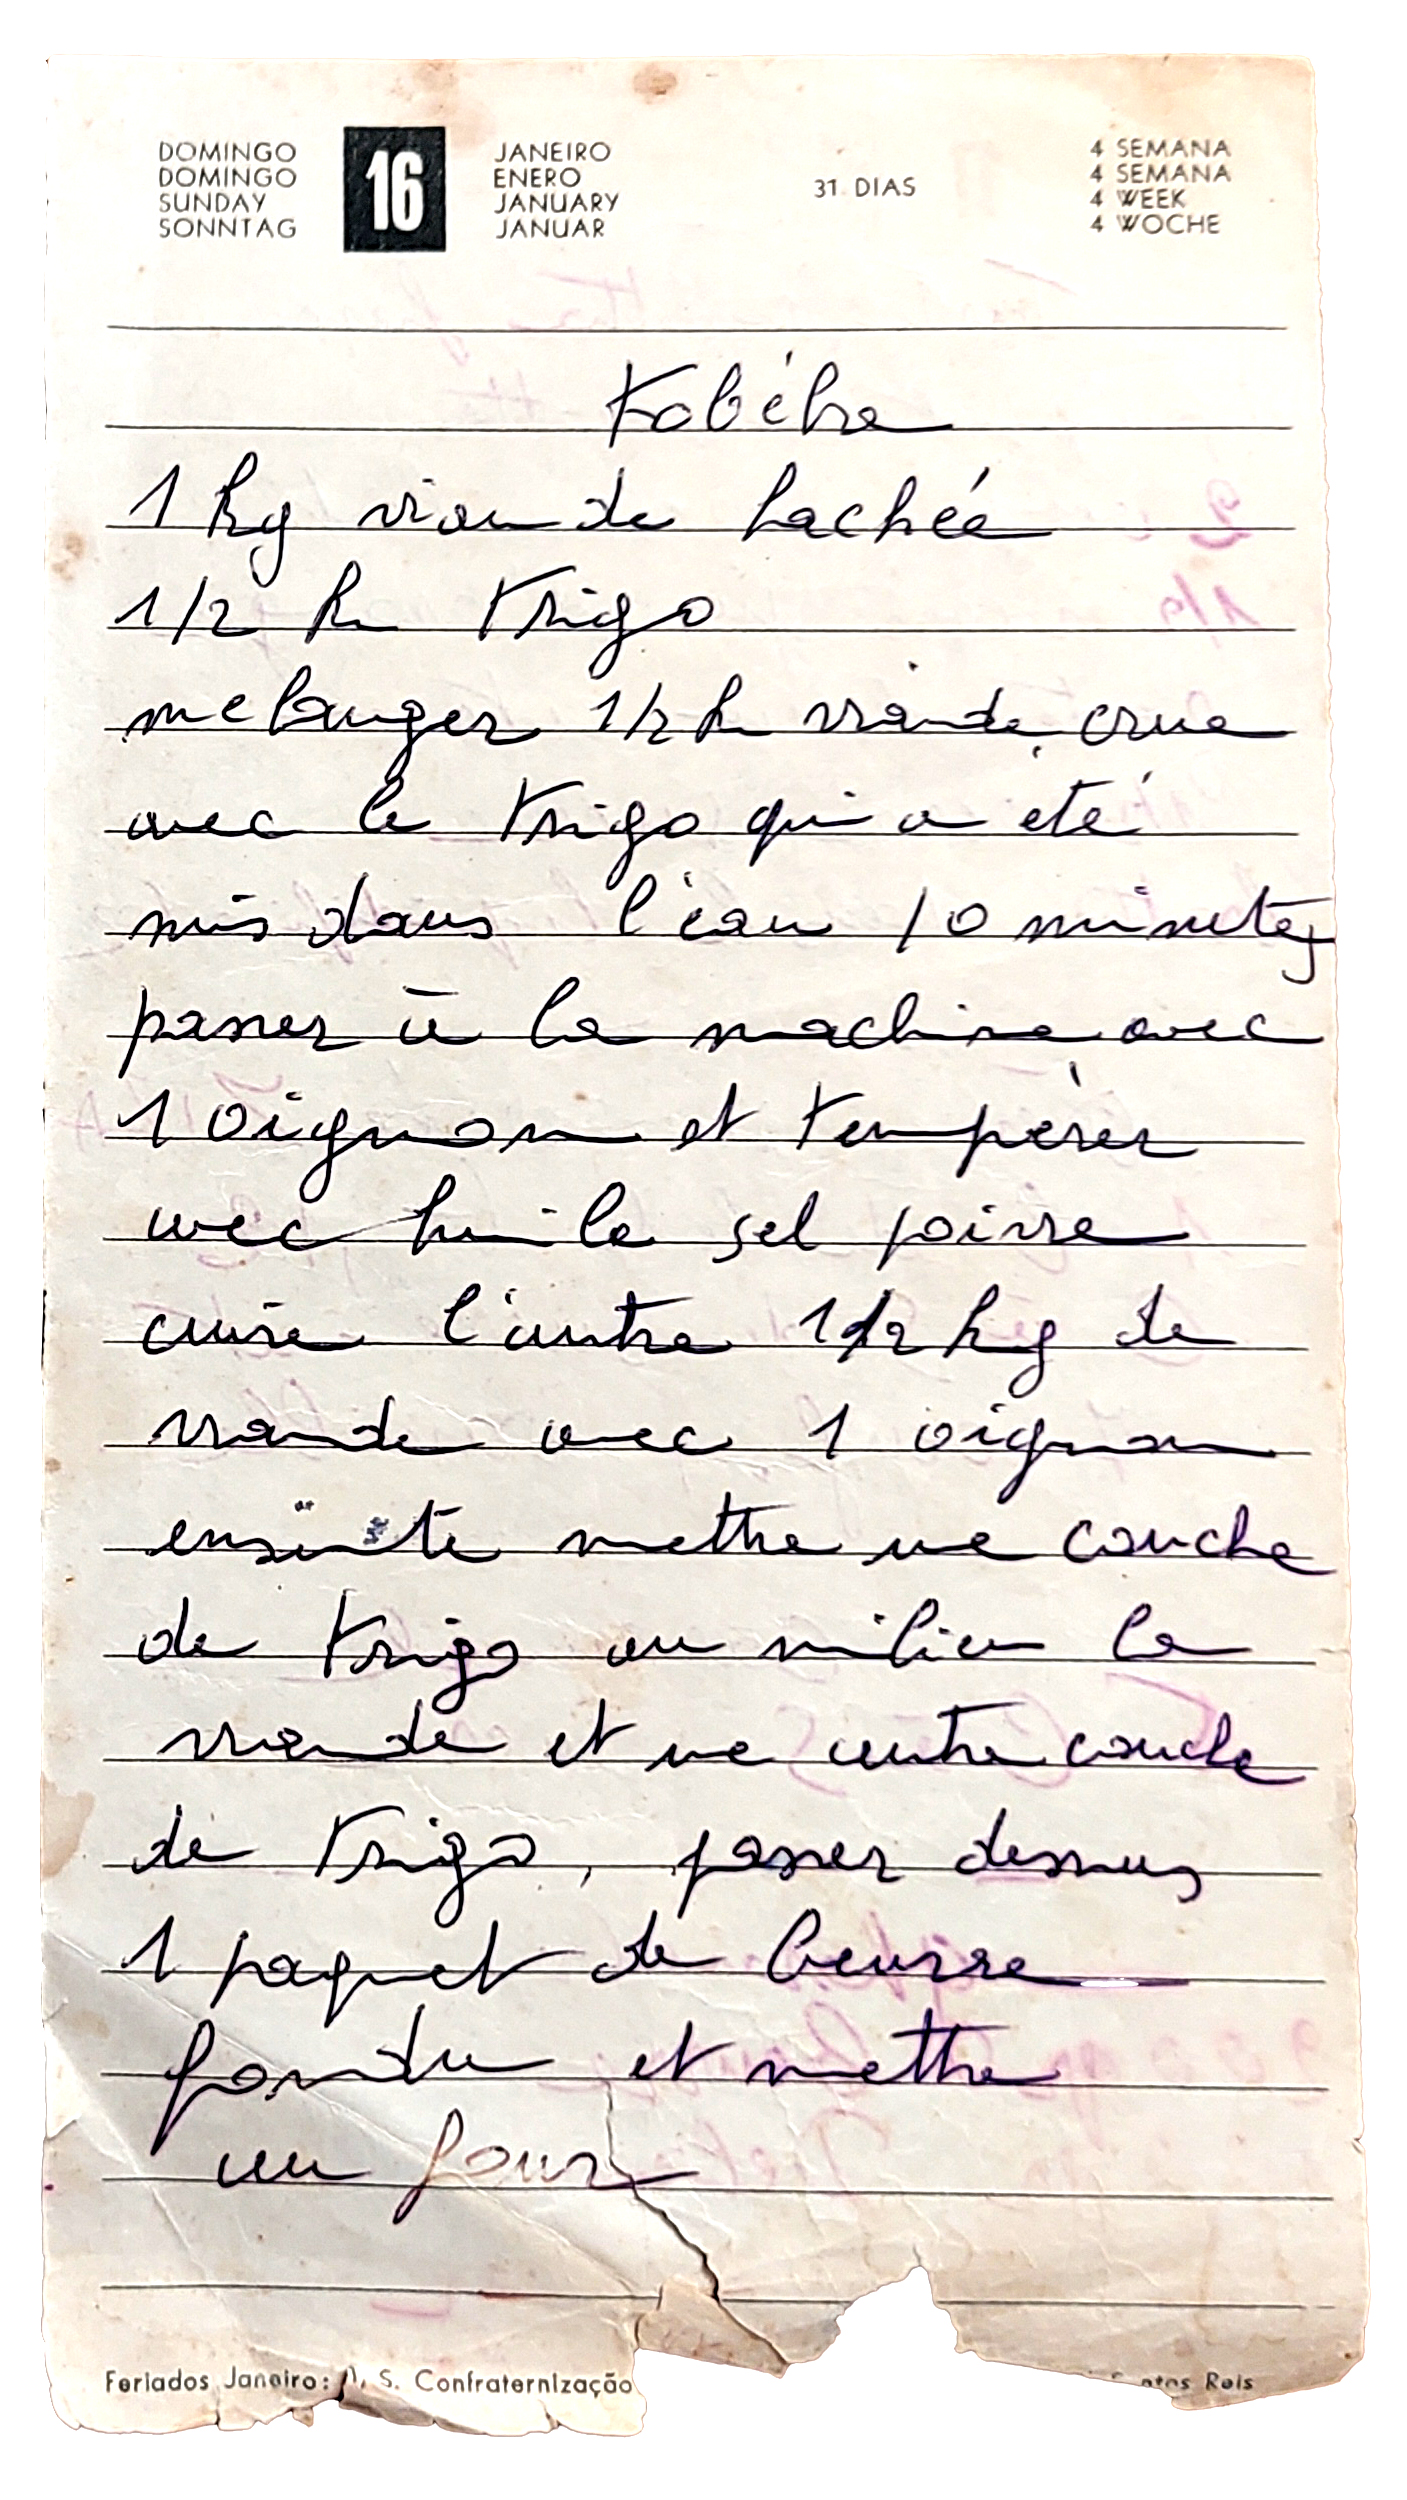
\includegraphics[width=8cm]{./recettes/edités/Kobéba.jpg}}; 
\end{tikzpicture}\clearpage\thispagestyle{empty}
% \begin{tikzpicture}[remember picture,overlay]
% \fill[black] (-3,3.5) rectangle (14,-21.5);
% \end{tikzpicture}
\clearpage

\chapter*{Kobéba}

\section{Ingrédients originaux}

\begin{itemize}
\item 1 kg viande hachée
\item 1/2 kg trigo
\item 2 oignons
\item Huile, sel, poivre
\item 1 paquet de beurre
\end{itemize}

\section{Préparation adaptée}

Misturez 1/2 kg de viande crue avec le boulgour préalablement trempé dans l’eau pendant 10 minutes et bien égoutté. Passez ce mélange au hachoir (ou mixez-le) avec 1 oignon et assaisonnez avec de l’huile, du sel et du poivre jusqu’à obtenir une préparation homogène. À part, faites revenir l’autre 1/2 kg de viande avec 1 oignon haché, en assaisonnant selon votre goût. Dans un moule huilé, étalez une couche de ce mélange de viande et de boulgour, ajoutez la viande cuite au centre puis recouvrez avec une seconde couche en lissant bien. Découpez en losanges ou en carrés, arrosez de beurre fondu et faites cuire au four préchauffé à 180°\,\textsc{c} pendant environ 30 à 40 minutes, jusqu’à ce que le dessus soit bien doré.

\chapter{Kobeba}

\section{Ingredientes originais}

\begin{itemize}
\item 1 kg de carne moída
\item 1/2 kg de trigo
\item 2 cebolas
\item Óleo, sal, pimenta
\item 1 tablete de manteiga
\end{itemize}

\section{Modo de preparo adaptado}

Misture 1/2 kg de carne crua com o trigo previamente hidratado em água por 10 minutos e bem escorrido. Passe essa mistura no moedor (ou processe) com 1 cebola e tempere com óleo, sal e pimenta até obter uma preparação homogênea. À parte, refogue o outro 1/2 kg de carne com 1 cebola picada, temperando a gosto. Em uma forma untada, espalhe uma camada dessa mistura de carne e trigo, adicione a carne cozida no centro e cubra com outra camada, alisando bem. Corte em losangos ou quadrados, regue com manteiga derretida e leve ao forno preaquecido a 180°\,\textsc{c} por cerca de 30 a 40 minutos, até que a superfície esteja bem dourada.